As mentioned in \autoref{sec:design-and-system-architecture}, the software for the system is written in Python and is run entirely on the Raspberry Pi 4B. The software is divided into three main components: the user interface, the computer vision system, and the system controller which manages the hardware components of the system. The software is designed to be modular, with each component being able to run independently of the others. This allows for easier debugging and testing of the system, as well as making it easier to add new features in the future. All written Python code adheres to a style defined in a \texttt{.pylintrc} file, which is a configuration file for the pylint \cite{pylint} linter. This ensures that the code is consistent and readable. The code is also documented using docstrings for readability and maintainability.

All software constants are defined in a \texttt{constants.py} file, which is imported by all other Python files, allowing for easy modification of constants that define the behaviour of the system which is useful for testing and debugging.

Additionally, a lot of thought went into streamlining the development process to ensure that the system is easy to develop and maintain. For example, Visual Studio Code's \cite{vscode} Remote SSH extension is used to develop the system remotely, as it allows developing the system on a much more powerful laptop, while using the familiar VSCode environment with any extensions that help streamline the development process. This is crucial as the Pi is not very powerful, so compiling and running the system on the Pi may be slow and cumbersome.

During development, the Pi connects to the laptop's Wi-Fi hotspot and is configured to be discoverable with the Pi's hostname, facilitating easy access to the Pi through SSH and a VNC Viewer without needing the Pi's IP address, which is dynamic. The Pi also makes use of SSH keys, allowing connection to the Pi without needing to enter a password every time, ensuring quick and easy access.

% Code block
\begin{minipage}[H]{\textwidth}
    \centering
    \begin{minted}[linenos, fontsize=\footnotesize, breaklines, bgcolor=bg]{python}
    # Allow development on non-Raspberry Pi devices
    try:
        import RPi.GPIO as GPIO # type: ignore
        RESIZEFLAG = False
        print("Using real hardware!")
    except ImportError:
        from src.common.simulate import GPIO
        RESIZEFLAG = True
        print("Simulating missing hardware!")
    \end{minted}
    \captionof{listing}{Cross-platform GPIO import}
    \label{code:cross-platform-gpio}
\end{minipage}

Additionally, as development is done on both a Windows laptop and the Pi, the code is written to be cross-platform, however certain libraries like the GPIO library are only available on the Pi, so a \texttt{simulate.py} file is used to simulate the GPIO pins on the laptop, allowing for development of the system without needing to be on the Pi as shown in \autoref{code:cross-platform-gpio}.

% Code block
\begin{minipage}[H]{\textwidth}
    \centering
    \begin{minted}[linenos, fontsize=\footnotesize, breaklines, bgcolor=bg]{python}
    # Allow development on non-Raspberry Pi devices
    class GPIO:
    BCM = 0
    IN, OUT = 0, 0
    HIGH, LOW = 0, 0
    PUD_DOWN, PUD_UP = 0, 0
    FALLING, RISING = 0, 0
    def setmode(_) -> None: pass
    def setup(_, *__, **___) -> None: pass
    def cleanup() -> None: pass
    def output(_, __) -> None: pass
    def add_event_detect(_, *__, **___) -> None: pass
    # PWM emulation
    class PWM:
        def __init__(self, _, __) -> None: pass
        def stop(self) -> None: pass
        def start(self, _) -> None: pass
        def ChangeDutyCycle(self, _) -> None: pass
        def ChangeFrequency(self, _) -> None: pass
    \end{minted}
    \captionof{listing}{Example simulation of the GPIO library}
    \label{code:simulate-gpio}
\end{minipage}

As shown in \autoref{code:simulate-gpio}, the \texttt{simulate.py} file contains a class called \texttt{GPIO} that emulates the GPIO library.

The Pi uses Git \cite{git} for version control, and the repository is hosted on GitHub \cite{github}, with a dedicated branch for the Pi that is regularly updated with the main branch. The vision system and the laptop also maintain their own Git branches which are regularly updated with the main branch, ensuring that all systems are running the same code. This is crucial as it enables development on a more powerful laptop, and then synchronises the changes to the Pi, without having to manually copy any files over. The repository can be found in the Appendix \ref{app:github}.
\subsubsection{User Interface}
The user interface allows the user to view and command the state of the system by interacting with the touchscreen on the DFRobot 7" display. From here, the user is able to\dots

\begin{figure}[H]
    \hfill
    \begin{minipage}[t]{\textwidth}
      \centering
      \includegraphics[height=8cm]{example-image-a}
      \caption{User Interface}
      \label{fig:ui}
    \end{minipage}
\end{figure}

As shown in \autoref{fig:ui}, the user interface consists\dots

Written in pygame \cite{pygamedoc} and pygame\_gui \cite{pygamegui}, the user interface is controlled by the \texttt{LCD UI} class, which is responsible for drawing the various elements of the user interface, such as the camera feed, the buttons, and the text. The system operates at 30Hz, allow for responsiveness without overloading the system. A profiler was used to determine the performance of the system, and it was found that the system was able to run at 30Hz without any issues as discussed in \autoref{sec:evaluation}.

The user interface also supports a "training mode", where the camera feed is enlarged in order to capture images of components to be used for training the computer vision system, done programmatically by toggling a flag called \texttt{TRAININGMODE} in the \texttt{LCD UI} class. This is only used during the dataset collection phase of the project, and is not used during the normal operation of the system. This is discussed in more detail in \autoref{sec:dataset-collection}.

\begin{figure}[H]
    \hfill
    \begin{minipage}[t]{\textwidth}
      \centering
      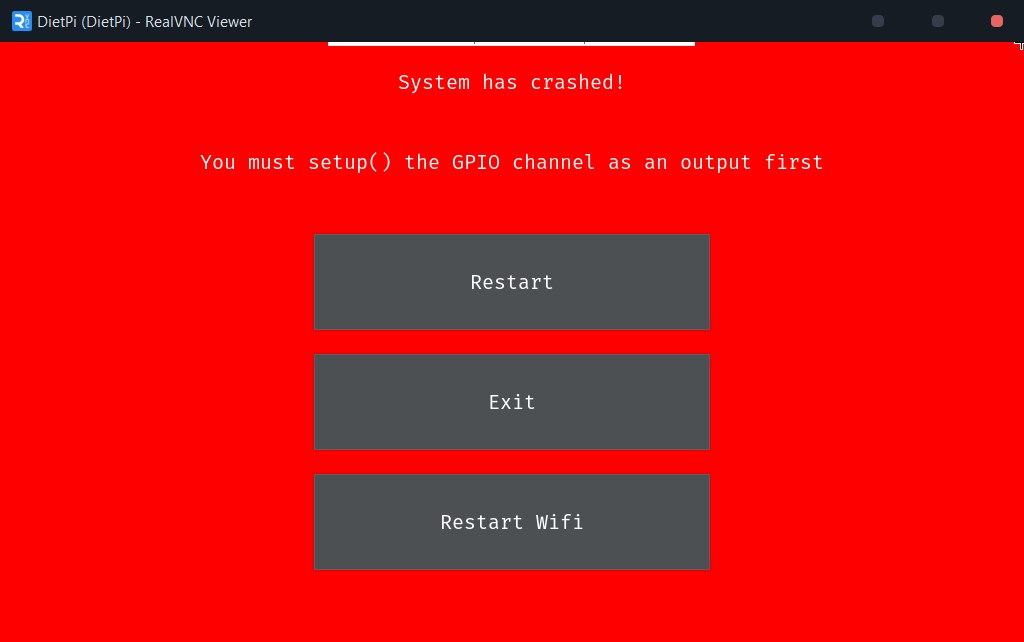
\includegraphics[height=8cm]{imgs/python/systemcrash.jpg}
      \caption{System crash during development}
      \label{fig:crash}
    \end{minipage}
\end{figure}

The LCD UI class is also capable of gracefully handling errors that may occur during the operation of the system, and the handling of these errors is delegated to the specific subsystem that caused the error. If a much more catastrophic error occurs, the system will still gracefully display an error screen, and allow the system to be restarted as shown in \autoref{fig:crash}. This facilitates not only the development process, but also prevents the system from having downtime in real-world applications as it prevents the need for a system restart. This is implemented by making use of Python's exception handling mechanism, and then switching to the error screen if an exception is raised.

The camera feed in the top left is controlled by the Vision Handler, which is responsible for delivering frames to the user interface. The Vision Handler is discussed in more detail in \autoref{sec:vision-handler}. 
\todo{Complete section after fully implementing the user interface}

\subsubsection{Vision Handler}
\label{sec:vision-handler}
The Vision Handler is responsible for managing the camera feed, and performs the following tasks:
\begin{mylist}
    \item Capturing frames from the camera
    \item Performing inference by passing the frames to the computer vision model
    \item Gracefully handling errors that may occur during inference
    \item Gracefully handling capture errors (such as the camera being disconnected)
    \item The ability to live capture from the \texttt{TRAININGMODE=True} UI mode to allow for development off the Raspberry Pi
\end{mylist}

\autoref{fig:camera-disconnect} shows what the user interface displays when the camera is disconnected.

\begin{figure}[H]
    \hfill
    \begin{minipage}[t]{\textwidth}
      \centering
      \includegraphics[height=8cm]{example-image-b}
      \caption{Camera disconnect error}
      \label{fig:camera-disconnect}
    \end{minipage}
\end{figure}

\subsubsection{System Controller}
\label{sec:system-controller}
\todo{diagram of interupt/data flow?}
The System Controller heavily leverages Python's \texttt{Multiprocessing} library to allow for the system to run multiple processes concurrently, allowing for the system to be more responsive while displaying the \texttt{LCD UI}. The System Controller is responsible for the following tasks:

\begin{mylist}
    \item Detecting a beam break and triggering procedure to sort the component
    \item Coordinating the movement of the \texttt{Sweeper Controller} to sort the component
    \item Relaying information back to the \texttt{LCD UI} to display the current state of the system
    \item Handling the event of the beam break sensor being triggered while the system is in the process of sorting a component
\end{mylist}

\todo{finish section}

\subsubsection{Dataset Collection}
\label{sec:dataset-collection}
As mentioned in \autoref{sec:data-annotation-tool}, a custom dataset annotation tool was used to collect and annotate the dataset required to train the YOLO-OBB model used for component identification, and then extended to train a regular YOLO model for resistor value detection.

\begin{figure}[H]
    \hfill
    \begin{minipage}[t]{\textwidth}
      \centering
      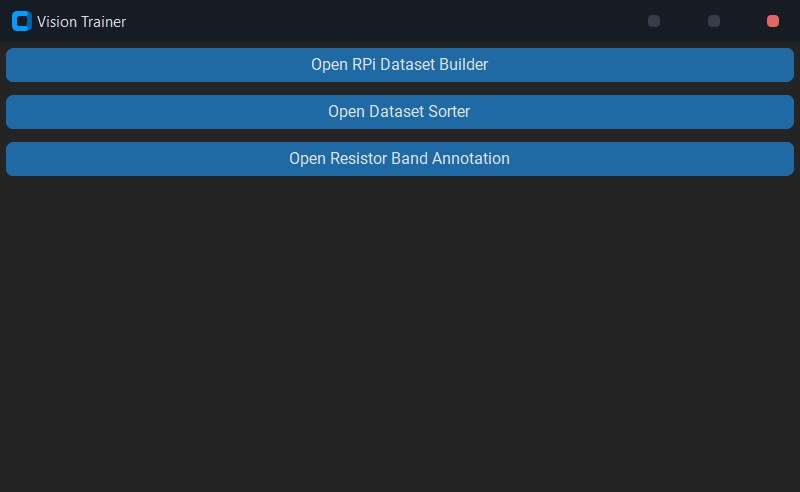
\includegraphics[height=8cm]{imgs/python/visiontrainer.jpg}
      \caption{Vision Trainer Menu}
      \label{fig:vision-trainer}
    \end{minipage}
\end{figure}

Upon launch, the user is able to select which mode they would like to use, as shown in \autoref{fig:vision-trainer}. The user can select the mode by using the following buttons:

\begin{table}[H]
    \centering
    \begin{tabularx}{0.8\textwidth}{|p{3cm}|X|}
        \hline
        \textbf{Button} & \textbf{Action} \\
        \hline
        \oldtexttt{RPi Dataset Builder} & Opens the dataset collection tool, capturing images from the VNC window connected to the Pi \\
        \hline
        \oldtexttt{Open Dataset Sorter} & Opens the dataset sorter tool that sorts a local dataset and reads the labels if they exist \\
        \hline
        \oldtexttt{Open Resistor Band Annotation} & Opens the resistor band annotation tool \\
        \hline
    \end{tabularx}
    \caption{Main buttons for the dataset collection tool}
    \label{tab:dataset-buttons}
\end{table}

\begin{figure}[H]
    \hfill
    \begin{minipage}[t]{\textwidth}
      \centering
      \includegraphics[height=8cm]{example-image-c}
      \caption{Training mode screen}
      \label{fig:training-mode}
    \end{minipage}
\end{figure}

As shown in \autoref{fig:training-mode}, to facilitate the collection of the dataset, the user interface was modified to include a "training mode" that allows the user to capture images of components to be used for training the computer vision system. As the camera feed must originate from the Pi, dataset collection is done on a machine connected to the Pi with VNC \cite{realvnc}, and the user interface is displayed on the VNC client. When \texttt{TRAININGMODE} is enabled, a purple border surrounds the camera feed, enabling the dataset tool to identify where the camera feed is located on the VNC window.

The tool makes use of keybinds to capture images, to allow the user to capture images of components quickly, detailed in the \autoref{tab:keybinds}.

\begin{table}[H]
    \centering
    \begin{tabularx}{0.8\textwidth}{|p{3cm}|X|}
        \hline
        \textbf{Key} & \textbf{Action} \\
        \hline
        \oldtexttt{Space} & Capture from VNC window \\
        \hline
        \oldtexttt{Enter} & Save image but only if the image is captured and labelled \\
        \hline
        \oldtexttt{Escape} & Return to the component selection screen \\
        \hline
        \oldtexttt{Mouse Left Click} & Draw line for OBB \\
        \hline
        \oldtexttt{Mouse Middle Click} & Cancel OBB \\
        \hline
    \end{tabularx}
    \caption{Main keybinds for the dataset collection tool}
    \label{tab:keybinds}
\end{table}

The dataset collection tool uses PyGetWindow \cite{pygetwindow_2020} to identify the VNC window, and PyAutoGUI \cite{pyautogui_2023} to capture the images. OpenCV's \cite{home_2024} \texttt{cv2.findContours} function is used to find the largest contour within the image that is bordered by the purple rectangle, allowing it to effectively extract the camera feed from the VNC window.

% Code block
\begin{minipage}[H]{\textwidth}
    \centering
    \begin{minted}[linenos, fontsize=\footnotesize, breaklines, bgcolor=bg]{python}
    try:
        realVNCWindow = pygetwindow.getWindowsWithTitle(REALVNC_WINDOW_NAME)[0]
        realVNCWindow.activate()
        pygetwindow.getWindowsWithTitle("RPi Dataset Builder")[0].activate()
    except:
        try:
            realVNCWindow = pygetwindow.getWindowsWithTitle("Component Sorter")[0]
            realVNCWindow.activate()
            pygetwindow.getWindowsWithTitle("RPi Dataset Builder")[0].activate()
        except:
            self.imgBorder.configure(bg_color=BORDER_COLOUR_FAILED)
            print("No Window Found")
            return
    # Capture the image
    screenshotPil = pyautogui.screenshot(region=(realVNCWindow.left, realVNCWindow.top, realVNCWindow.width, realVNCWindow.height))
    # Convert to OpenCV format
    screenshotCv = numpy.array(screenshotPil)
    # Find the contours defined by the pink square
    mask = cv2.inRange(cv2.cvtColor(screenshotCv, cv2.COLOR_BGR2HSV), LOWER_THRESHOLD, UPPER_THRESHOLD)
    contours, _ = cv2.findContours(mask, cv2.RETR_TREE, cv2.CHAIN_APPROX_SIMPLE)
    \end{minted}
    \captionof{listing}{Camera feed extraction from VNC window}
\end{minipage}

\begin{figure}[H]
    \hfill
    \begin{minipage}[t]{\textwidth}
      \centering
      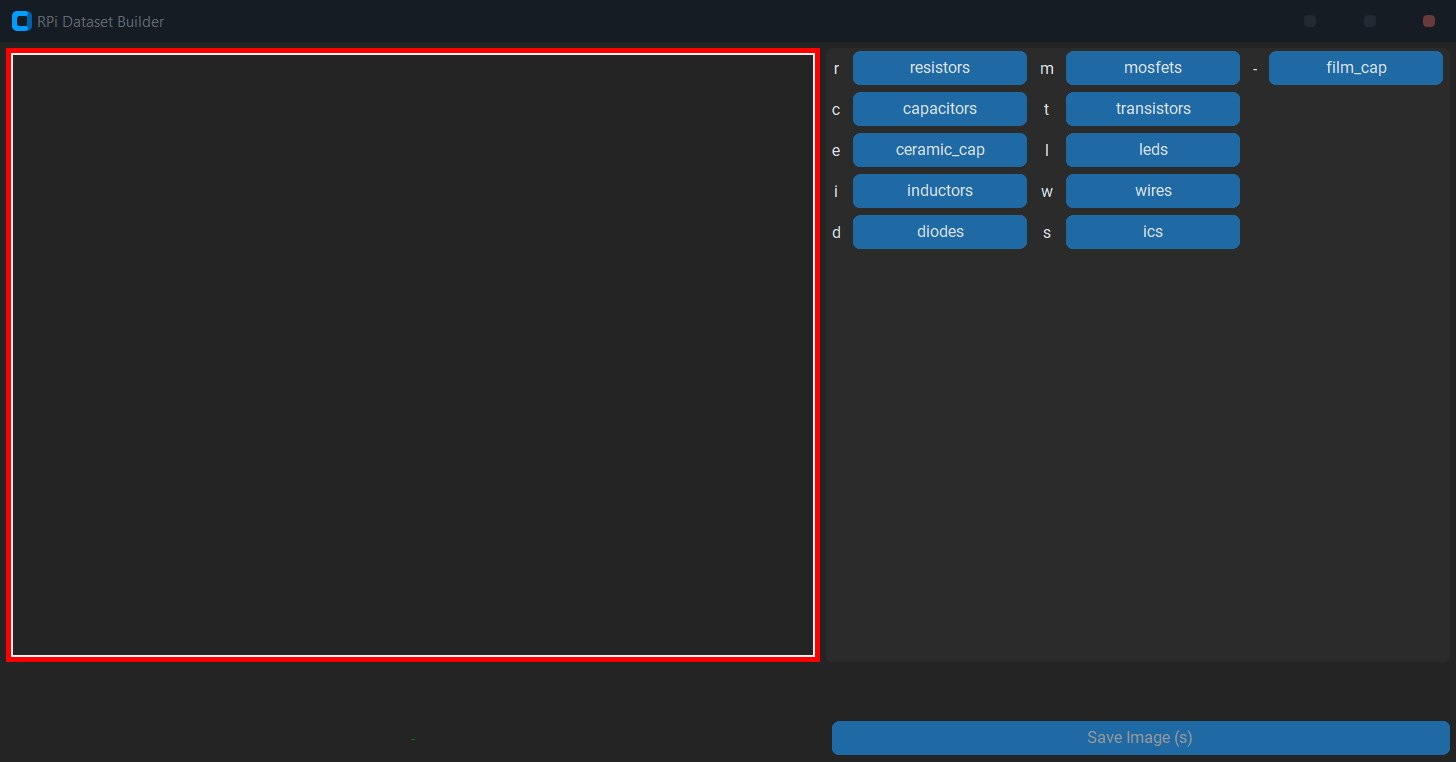
\includegraphics[height=8cm]{imgs/python/uncaptured.jpg}
      \caption{Uncaptured camera feed with red border}
        \label{fig:uncaptured}
    \end{minipage}
\end{figure}

If the camera feed is not captured (it may be obscured), the border of the camera feed will turn red, as shown in \autoref{fig:uncaptured}, indicating that the camera feed was not captured, otherwise it will turn green, as shown in \autoref{fig:captured}. In \autoref{fig:uncaptured}, the user is selecting which component to sort on the component selection screen, and has a selection from the following components: 
\begin{multicols}{2}
    \begin{mylist}
        
        \item Resistors
        \item Capacitors
        \item Ceramic Capacitors
        \item Inductors
        \item Diodes
        \item MOSFETs
        \item Transistors
        \item LEDs
        \item Wires
        \item ICs
        \item Film Capacitors
    \end{mylist}
\end{multicols}

The user can select the component to sort by clicking on the component button or by using the hotkey indicated to the left of the button.  

\begin{figure}[H]
    \hfill
    \begin{minipage}[t]{\textwidth}
      \centering
      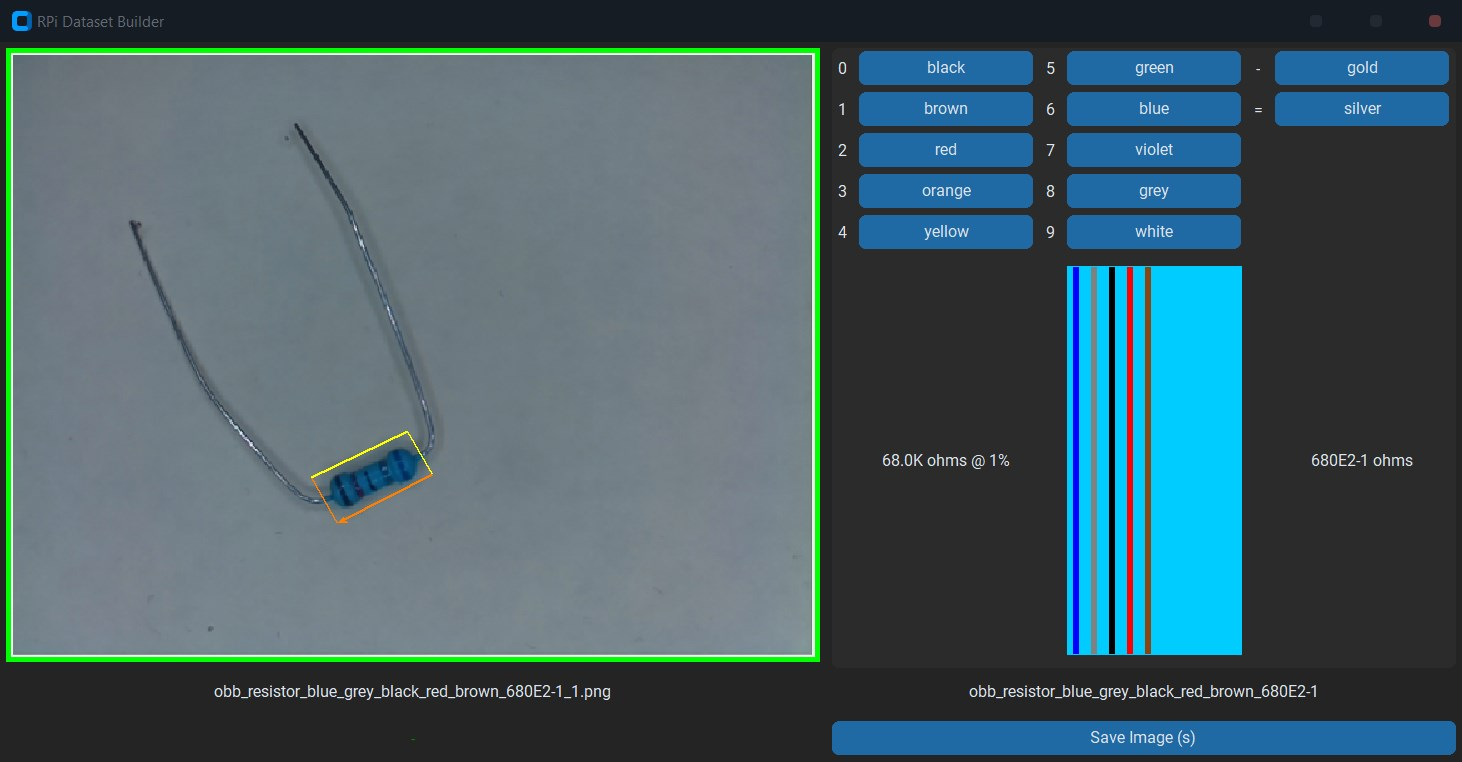
\includegraphics[height=8cm]{imgs/python/captured.jpg}
      \caption{Successfully captured camera feed with green border and annotated resistor}
        \label{fig:captured}
    \end{minipage}
\end{figure}

In \autoref{fig:captured}, the user has successfully captured the camera feed, and has annotated a resistor. The tool has hotkeys for quickly annotating the band and retains the configuration of the band between images, allowing for quick annotation of resistors (as the user would take multiple angles of the same resistor). During band annotation, the program automatically calculates what the value of the resistor should be, including tolerances, and displays this on the screen, to help prevent the mislabelling of the resistors. The bands and value are then saved in the filename of the image and label, allowing the resistor value model to be trained based off the file names. For eaxmple, in \autoref{fig:captured}, the resistor will be saved as \texttt{obb\_resistor\_blue\_grey\_black\_red\_brown\_680E2-1\_1.png}; the value of the resistor is 68 k$\Omega$, with a tolerance of 1\% and is the first image of this value in the dataset.

The user can also draw the OBB by clicking and dragging the mouse, and can cancel the OBB by clicking the middle mouse button. The tool automatically connects the first and last points to form the OBB, showing a gray dotted line so the user can verify the OBB is correct. The user can then save the image by pressing the \texttt{Enter} key, or return to the component selection screen by pressing the \texttt{Escape} key.

Originally, it was thought that the OBB model learns the correct left-right orientation of objects by the order of which the vertexes are joined, and this is represented in the tool with two orange arrows, showing the desired right-side up orientation of the resistor. However, this was found to be incorrect, and the OBB model only learns the bounding box of the object, and not the orientation of the object. This was discovered during the training of the OBB model, as discussed in \autoref{sec:computer-vision}

\begin{figure}[H]
    \hfill
    \begin{minipage}[t]{0.45\textwidth}
      \centering
      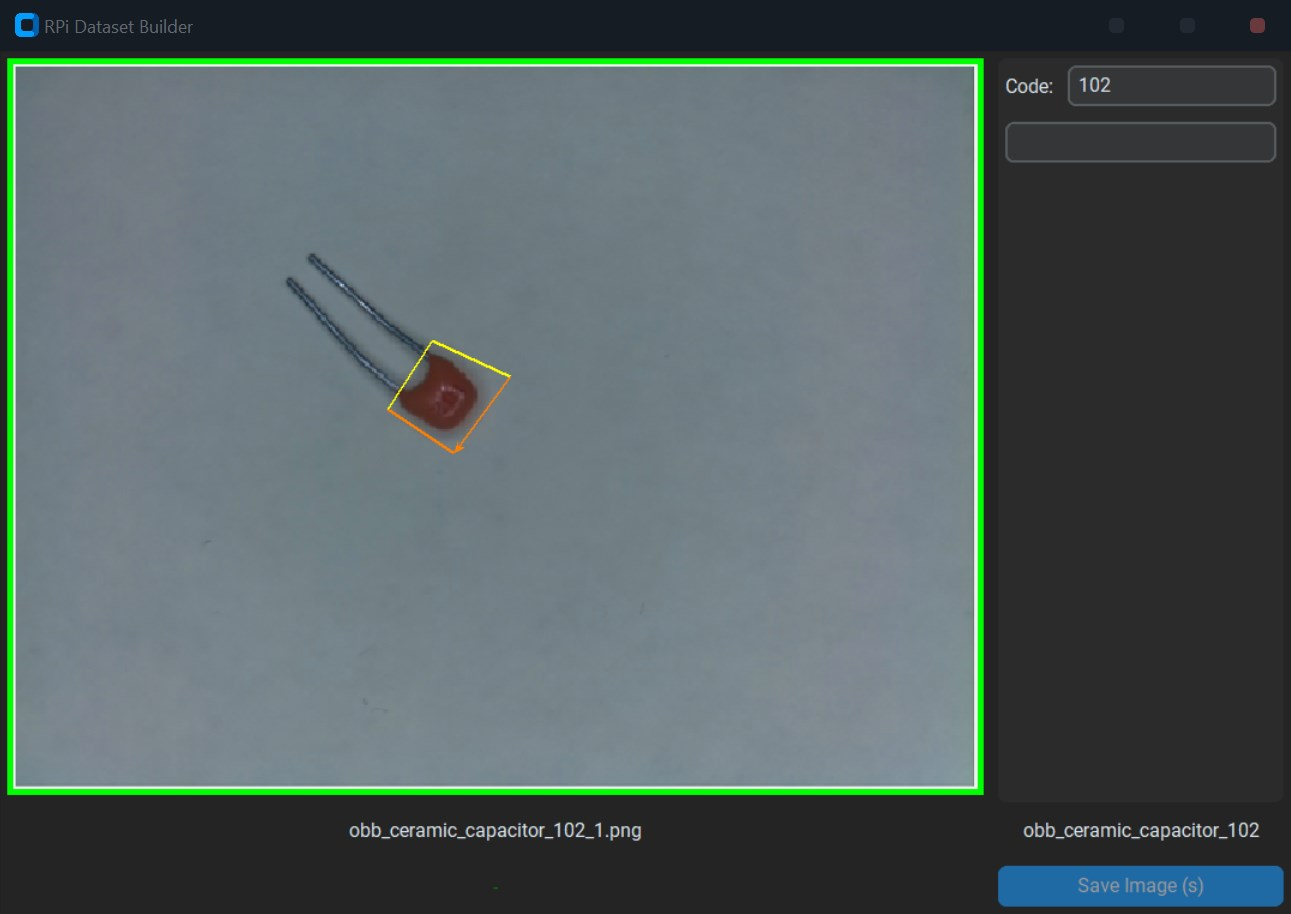
\includegraphics[width=\columnwidth]{imgs/python/capcapture.jpg}
      \caption{Annotated Ceramic Capacitor}
      \label{fig:capcapture}
    \end{minipage}
    \hfill
    \begin{minipage}[t]{0.45\textwidth}
      \centering
      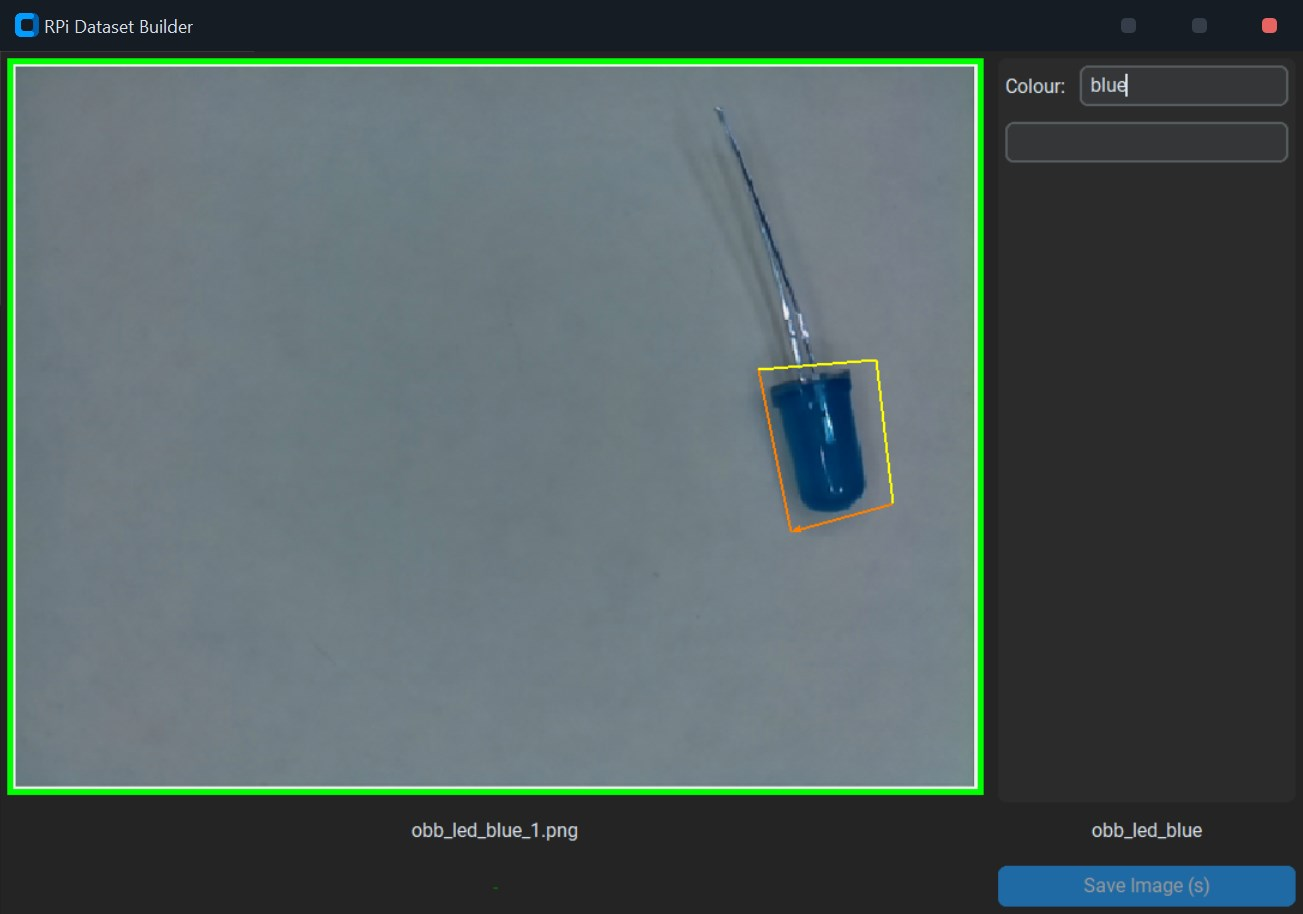
\includegraphics[width=\columnwidth]{imgs/python/ledcapture.jpg}
      \caption{Annotated LED}
      \label{fig:indcapture}
    \end{minipage}
    \hfill
\end{figure}

\autoref{fig:capcapture} shows an annotated ceramic capacitor, and \autoref{fig:indcapture} shows an annotated LED, demonstrating the tool's ability to annotate components of different shapes and sizes.

In addition to regular component identification using the YOLO-OBB model, a separate model was trained to identify the value of resistors, which is discussed in more detail in \autoref{sec:computer-vision}. This dataset is collected by using the classification model to identify the resistor, and then the bounding box is used to crop the image to the resistor. The cropped image then contains the neccessary information to train the resistor value model, such as the bands and the value of the resistor, but is missing the location of the bands in the image, and the orientation of the resistor, which would help it determine what the first band is. This means a tool is still required to annotate the resistor bands.

\begin{figure}[H]
    \hfill
    \begin{minipage}[t]{\textwidth}
      \centering
      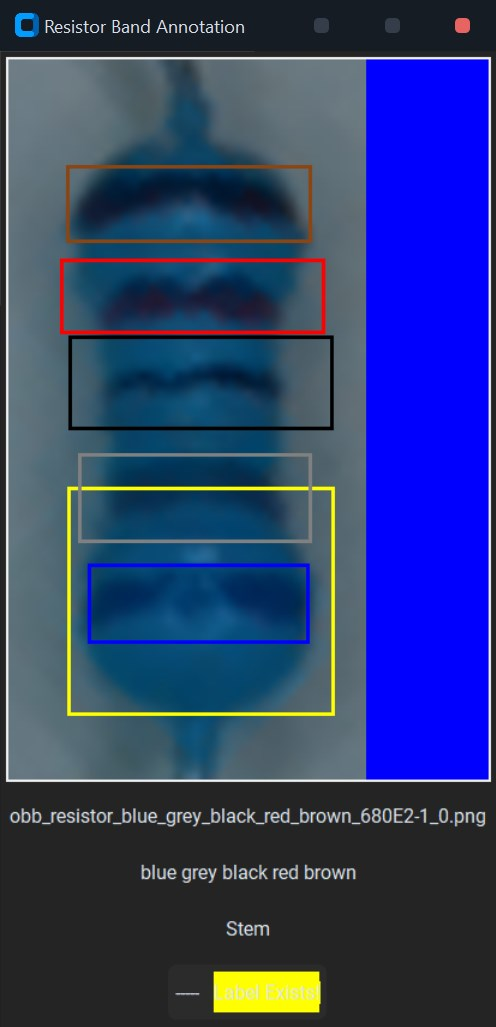
\includegraphics[height=8cm]{imgs/python/resistorannotate.jpg}
        \caption{Resistor band annotation tool}
        \label{fig:resistorannotate}
    \end{minipage}
\end{figure}

As shown in \autoref{fig:resistorannotate}, the tool clearly shows a resistor being annotated, with the bands being drawn on the resistor. The user only has to click on the location of the bands, and does not need to manually annotate what band the user is clicking on; the information of the order of the bands in encoded in the filename as discussed earlier, so the tool can automatically determine what band the user is clicking on. The user only needs to indicate where the 'stem' of the resistor is, indicated by the yellow box, enabling the tool to identify the orientation of the resistor, and then allowing the resistor value model to be trained. Clicking on the resistor automatically draws a bounding box centered at the band location with the current band colour, and then saves the image and label in the same way in the YOLO format (not the YOLO-OBB format as the component identification model will always produce resistors upright). The format is discussed in more detail in \autoref{sec:computer-vision}. 

